\documentclass[12pt,a4paper]{article}
\usepackage{geometry}
\geometry{margin=1in}
\usepackage{times}
\usepackage{graphicx}
\usepackage{fancyhdr}
\usepackage{hyperref}
\usepackage{titlesec}
\usepackage{float}      
\usepackage{placeins}   
\renewcommand{\textfraction}{0.05}
\renewcommand{\floatpagefraction}{0.9}
\renewcommand{\topfraction}{0.9}
\renewcommand{\bottomfraction}{0.9}
\graphicspath{{.}{./}{./figs/}} 
\pagestyle{fancy}
\fancyhf{}
\rhead{Operating Systems Project1}
\lhead{Yangyang Jiang}
\rfoot{\thepage}

\titleformat{\section}{\large\bfseries}{\thesection}{1em}{}
\titleformat{\subsection}{\normalsize\bfseries}{\thesubsection}{1em}{}

\begin{document}

\begin{titlepage}
    \centering
    \vspace*{3cm}
    {\Huge \textbf{Operating Systems Project1 Report}}\\[1.5cm]
    {\Large Process Scheduling Simulation}\\[1.5cm]
    \textbf{Course:} 4320/6320 -- Operating Systems (Fall 2025)\\[0.5cm]
    \textbf{Student:} Yangyang Jiang\\[0.5cm]
    \textbf{Github:} https://github.com/techyangj/operation-system-project-1\\[0.5cm]
    \vfill
    \vfill
\end{titlepage}

\section{Introduction}
This project implemented a process scheduling simulation in \textbf{C}. The goal was to simulate how an operating system uses the CPU scheduling algorithm to schedule processes. The process scheduler determines which process runs on the CPU at a given time. This project allowed me to learn how real operating systems handle CPU scheduling, furthering my understanding of how operating systems work. 

This program reads processes from the input file \textbf{processes.txt}, schedules them according to the selected scheduling algorithm, and outputs the wait time (WT), turnaround time (TAT), completion time (C) of each process, as well as the averages and the corresponding Gantt chart.

The implemented two algorithms are:
\begin{itemize}
    \item \textbf{First-Come, First-Served (FCFS)}
    \item \textbf{Shortest Job First (SJF, non-preemptive)}
\end{itemize}

\section{Implementation Details}

\subsection{Input Handling}
Processes are defined in a text file with four fields: \textbf{PID, Arrival Time, Burst Time, and Priority.} 
Lines are parsed into an array of \textbf{struct Process}. Empty lines and comments are skipped.

\subsection{Command-Line Arguments}
The program supports flexible execution using command-line arguments:
\begin{itemize}
    \item \texttt{-h} or \texttt{--help} \quad Displays usage information.
    \item \texttt{-a <algo>} \quad Selects the scheduling algorithm:
        \begin{itemize}
            \item \texttt{fcfs} -- Run only First-Come, First-Served
            \item \texttt{sjf} -- Run only Shortest Job First
            \item \texttt{both} -- Run both algorithms
        \end{itemize}
    \item \texttt{-f <file>} \quad Specify an input file (default: \textbf{processes.txt}).
\end{itemize}

I think users can quickly test different algorithms and datasets without recompiling or modifying the source code.

\subsection{FCFS}
\begin{itemize}
    \item Processes are sorted by arrival time, then by PID.  
    \item Each process runs in order of arrival.  
    \item CPU idle periods are recorded when no process has arrived.  
    \item For each process:  
        \begin{itemize}
            \item Completion Time $C = finish~time$
            \item Waiting Time $WT = start - arrival$
            \item Turnaround Time $TAT = C - arrival$
        \end{itemize}
\end{itemize}

\subsection{SJF (Non-Preemptive)}
\begin{itemize}
    \item At each decision point, the ready process with the shortest burst time is chosen.  
    \item Ties are resolved by arrival time, then by PID.  
    \item Idle segments are added if CPU is waiting for arrivals.  
    \item WT, TAT, and C are computed as in FCFS.  
\end{itemize}

\subsection{Gantt Chart}
Execution order is visualized as a text-based Gantt chart. For example:

\begin{verbatim}
| P1 | Idle | P2 | P3 |
0    2      5    7    10
\end{verbatim}

\section{Results}

\subsection{Command Argument}
\begin{figure}[h]
    \centering
    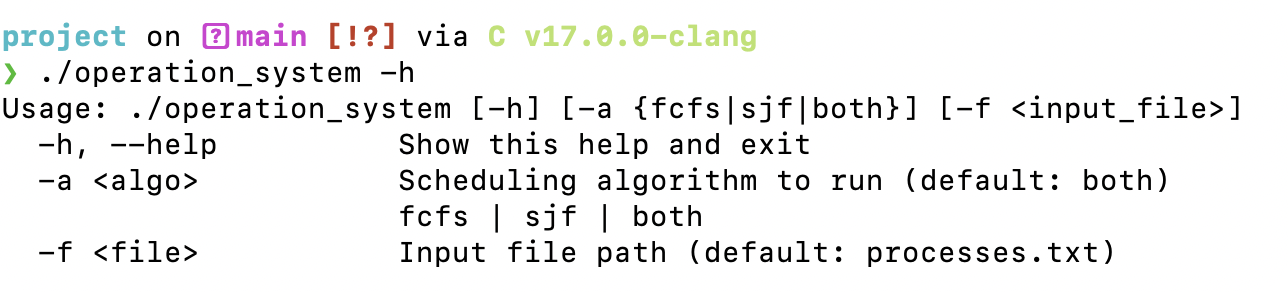
\includegraphics[width=0.9\linewidth]{h.png}
    \caption{Command Argument.}
\end{figure}
\subsection{Sample Input}
\begin{verbatim}
PID  Arrival_Time  Burst_Time  Priority
1    0             5           2
2    2             3           1
3    4             2           3
\end{verbatim}
\subsection{FCFS Output}
The following figure shows the detailed results of the FCFS scheduling algorithm,
including the process execution order and the corresponding Gantt chart.

\begin{figure}[H]
    \centering
    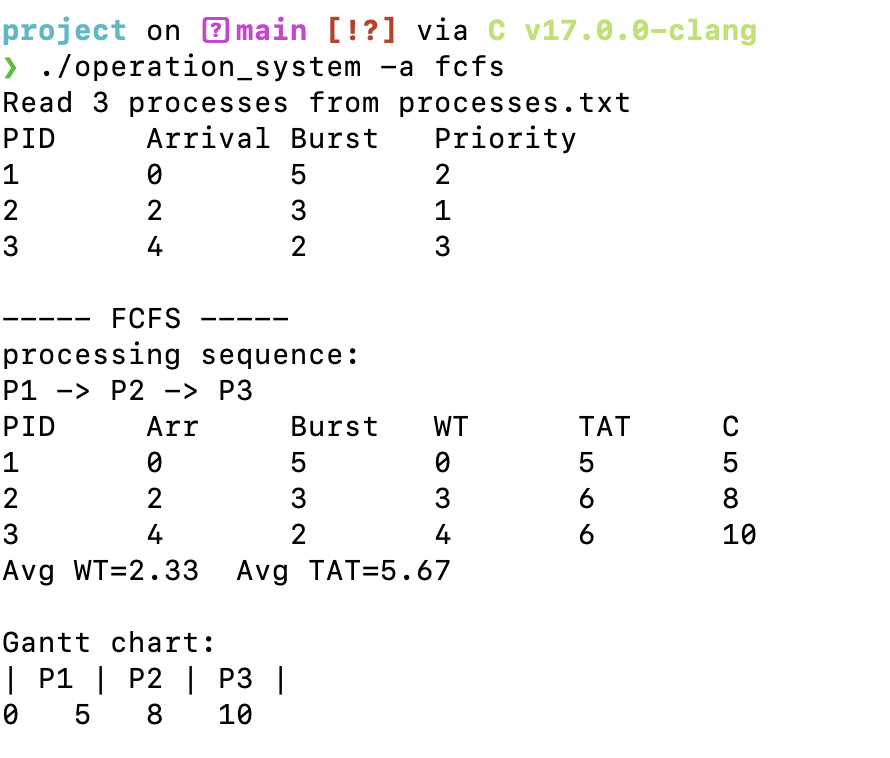
\includegraphics[width=\linewidth]{a_fcfs} 
    \caption{FCFS Processes and Gantt Chart for the sample workload.}
    \label{fig:fcfs}
\end{figure}
\FloatBarrier

\subsection{SJF Output}
The following figure illustrates the SJF (non-preemptive) scheduling results.
It shows how shorter jobs are scheduled earlier, reducing the average waiting time.

\begin{figure}[H]
    \centering
    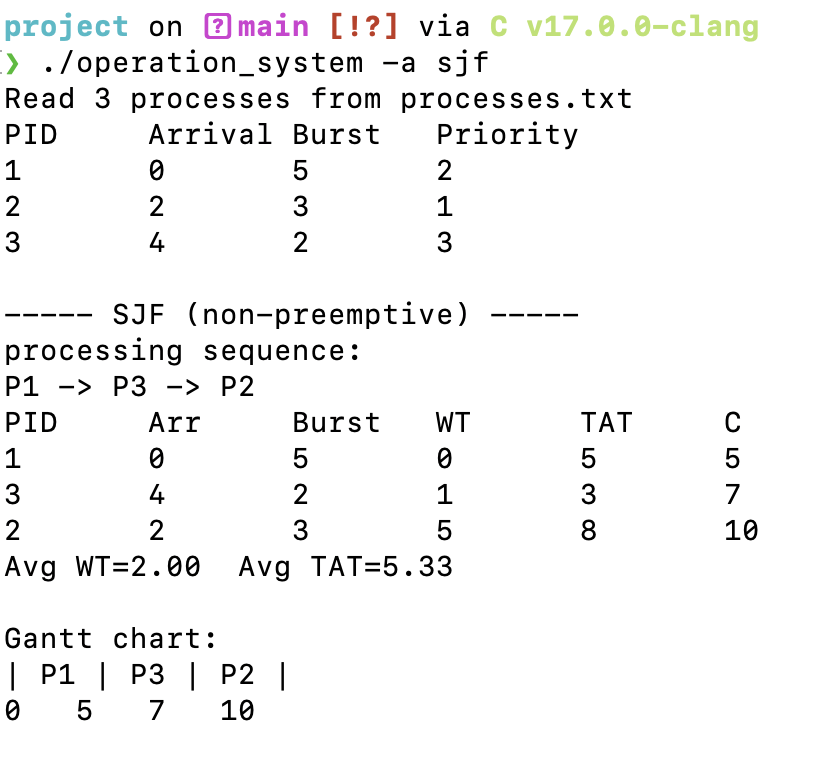
\includegraphics[width=\linewidth]{a_sjf}
    \caption{SJF Processes and Gantt Chart for the sample workload.}
    \label{fig:sjf}
\end{figure}
\FloatBarrier

\section{Analysis}
The FCFS scheduling algorithm is simple to implement using C code, but it has significant drawbacks. If a process takes a long time to execute, subsequent processes may continue to wait, ultimately leading to slackness. In contrast, the SJF scheduling algorithm prioritizes shorter jobs, effectively reducing average waiting time and turnaround time, resulting in better overall system performance than the FCFS scheduling algorithm.

\section{Challenges}
Implementing the SJF algorithm is significantly more difficult than the FCFS algorithm. Unlike FCFS, SJF requires checking which processes have reached their current time and then selecting the one with the shortest time. This is primarily due to the difficulty of tracking which processes have completed and which are still waiting. However, this problem is solved by maintaining the \texttt{done[]} array and carefully updating the timeline.
Optional memory management is difficult to extend. Using memory allocation requires introducing new data types and methods. The amount of code changes required is too large for the current stage of the project, so memory management is left for a later date.

\section{Conclusion}
This project successfully implemented and tested two CPU scheduling algorithms in C: FCFS and SJF.  

\begin{itemize}
    \item The program reads process data from a file, computes WT/TAT, and displays a Gantt chart.  
    \item FCFS is fair but can penalize shorter processes.  
    \item SJF optimizes average WT and TAT but assumes burst times are known in advance.  
\end{itemize}


\end{document}
